\section{Selection}

Signal candidates for the decays \btokpipimumu and \btophikmumu must first pass the \lone muon
trigger.
Subsequent software trigger stages required that at least one final-state muon has $\pt>1.6\gev$
and at least one hadron has $\pt>1.0\gev$, both of which had an IP larger than $100\mum$ with
respect to any PV in the event.
The response of the topological BBDT in the \hlttwo must be consistent with a decaying $B$ meson
with muons in the final state.

%There is large overlap between the...

Candidate \Bp hadrons are then formed from combinations of three hadrons and a pair of opposite
sign muons.
Fully reconstructed candidates must form a good quality vertex, with a \chisq of the vertex fit
$<6$.
This secondary vertex must be well displaced from any PV, having a flight distance inconsistent
with zero; ($\chisqfd>121$).
The angle between the \Bp candidate momentum vector and the direction defined by the PV to \Bp decay
vertex must be less than $14\mrad$.
Each track must satisfy $\chisqip>16$, where the \chisqip of a track is defined as the change in
\chisqip when calculated with and without the track in question.
The muons must both satisfy the {\tt isMuon} criteria and have $\dllmupi>0$.
Hadrons have PID criteria applied later, after optimization, but the total invariant mass of the
\kpipi system is required to be below $2400\mev$.
Each hadron must have $\pt>500\gev$.
For the \phik system, the additional constraint that the \decay{\phi}{\kk} object must have an
invariant mass within $12\mev$ of $m_\phi^\pdg$.

To change the signal yields into branching fractions normalization channels were needed.
The normalization channel for the decays \btokpipimumu and \btophikmumu are \btopsitwosk and
\btojpsiphik (where \psitwostojpsipipi and \jpsitomumu) respectively.
These are chosen to have the same final state particles as the signal decays to ensure that PID
efficiencies cancel.
The decay \btojpsikpipi is also used in this analysis for cross-checks and in training the BDT (as
described in \Sect{sec:hhh:bdt}).
All these decays were subject to the same selection criteria except for requirements on the
invariant mass of the dimuon pair.
For each \psitwos and \jpsi candidate, it is required that
$\big|m_{\mu\mu}-m_{\psitwos}^\pdg\big|<50\mev$ and
$\big|m_{\mu\mu}-m_\jpsi^\pdg\big|<50\mev$ respectively.


\begin{table}
  \caption{\small
    Requirements in the {\tt BuToK1MuMuLine} stripping line in {\tt Stripping20}.
    The variable {\tt ADOCACHI2CUT} is the \chisq distance of the closest approach
    (below a threshold) for all two particle combinations, and {\tt DIRA} is the
    angle between the reconstructed \Bp momentum and that from the hits in the
    \velo.
  }
  \label{tab:hhh:strip}
  \begin{center}
    \begin{tabular}{llcr}\toprule
      Particle & Variable & \multicolumn{2}{c}{Value} \\ \midrule
      $B$
      & \chisqvtx               &  $<$ & $6.0$ \\
      & \chisqip               &  $<$ & $16.0$ \\
      & \chisqfd               &  $>$ & $121.0$ \\\littlerule
      \kpipi
      & Vtx $\chi^2$  &  $<$ & $12.0$ \\
      & $\mathtt{\,DIRA}$    &  $>$ & $-0.9$ \\
      & \mass{\kpipi}          &  $\in$ & $[750, 2400]\mev$\\
      & ADOCACHI2CUT & $<$ & $ 20$ \\
      & \chisqip          &  $<$ & $4.0$ \\
      & \chisqfd            &  $>$ & $25.0$ \\\littlerule
      \mumu
      & \chisqvtx     &  $<$ & $12.0$ \\
      & \chisqfd                &  $>$ & $81.0$ \\
      tracks  & \chisqip     &  $>$ & $16.0$ \\
      & track $\chisq/$ndof         &   $<$ & $2.5$ \\\littlerule
      \Kp, \pip
      & $p_T$                  &   $>$ & $500$ \\
      \mup & \ismuon  \\
      \bottomrule
    \end{tabular}
  \end{center}
\end{table}




\subsection{Peaking backgrounds}
Processes with the same final state as \btokpipimumu and \btophikmumu are not smoothly distributed
in $m_{K\pi\pi\mu\mu}$, rather they peak under the signal.
The tree level decays \decay{\Bp}{\jpsi\kpipi} and \decay{\Bp}{\jpsi\phik}, where
\decay{\jpsi}{\mumu}, have large branching fractions:
\begin{align}
  \BF\big(\decay{\Bp}{\jpsi\kpipi}\big)
  \cdot \BF\big(\jpsitomumu\big)
  &= (4.8 \pm 0.8)\e{-5} \\
  \BF\big(\decay{\Bp}{\jpsi\phik}\big)
  \cdot \BF\big(\jpsitomumu\big)
  &= \big(3.1 \pm 1.1\big)\e{-6},
\end{align}
and the same final state particles.
The same is true for the large contributions from \decay{\Bp}{\psitwos\kpipi} and
\decay{\Bp}{\psitwos\phik} decays, where \decay{\psitwos}{\mumu}.
These contributions from charmonium decays constitute large, irreducible backgrounds and must be
removed with vetoes around the \jpsi and \psitwos masses.
The vetoes used remove events where the invariant dimuon mass falls in either region
$2946<m_{\mu\mu}<3176\mev$ or $3586<m_{\mu\mu}<3766\mev$.

Mis-reconstructed decays to charmonium contribute to the upper mass sideband.
To remove these, the veto windows are extended up by $40\mev$ in the region
$5330<m_{K\pi\pi\mu\mu}<5450\mev$.
Radiative tails from the decays \decay{\jpsi}{\mumu\gamma} and \decay{\psitwos}{\mumu\gamma} are
suppressed by extending the vetoes down by $250\mev$ and $100\mev$ respectively in the region
$m_{K\pi\pi\mu\mu}<5230\mev$.
Figure~{fig:hhh:charmvetoes} shows the boundaries defined by these vetoes on data.

%However, the amount of contamination from decaying \jpsi and \psitwos is so great that both show
%evidence of asymmetric tails from

\begin{figure}
  \begin{center}
    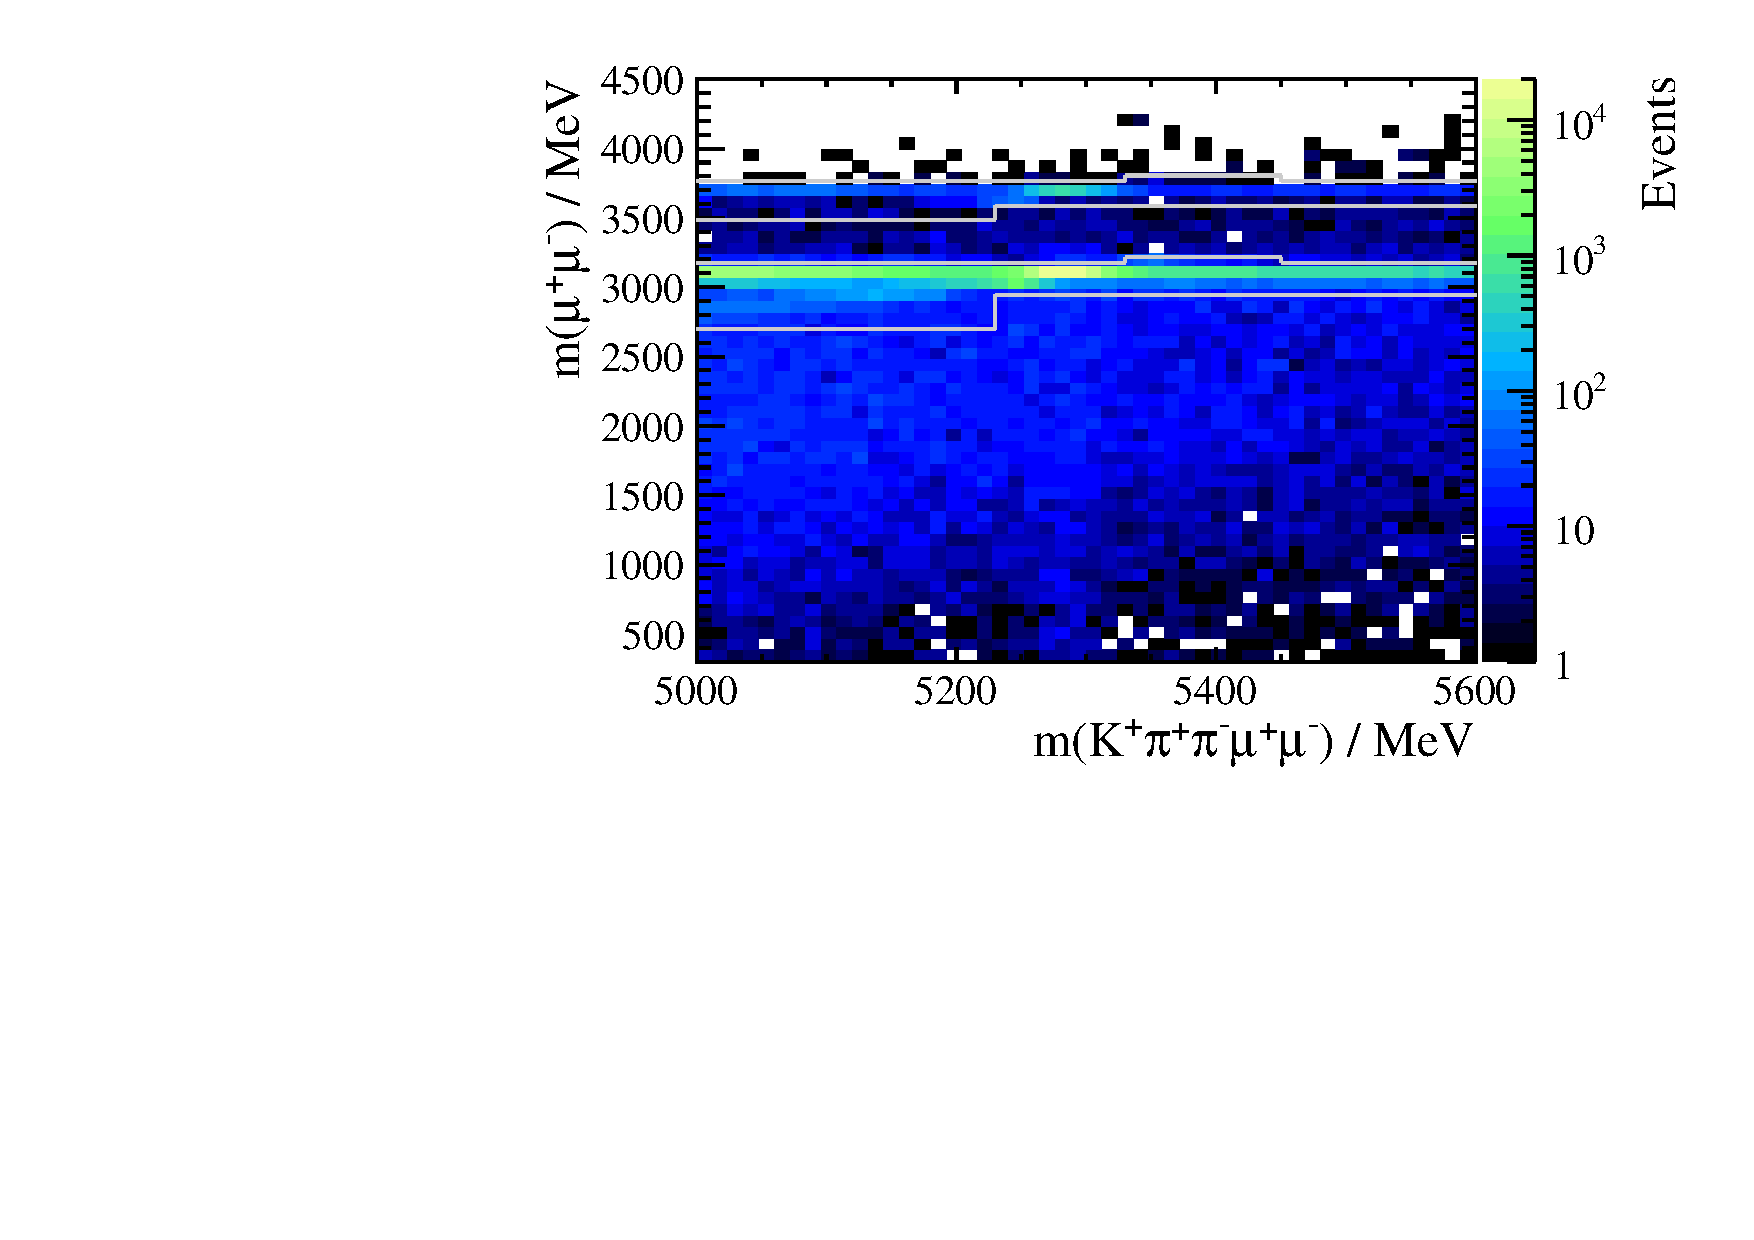
\includegraphics[width=0.48\textwidth]{BvJpre}
    %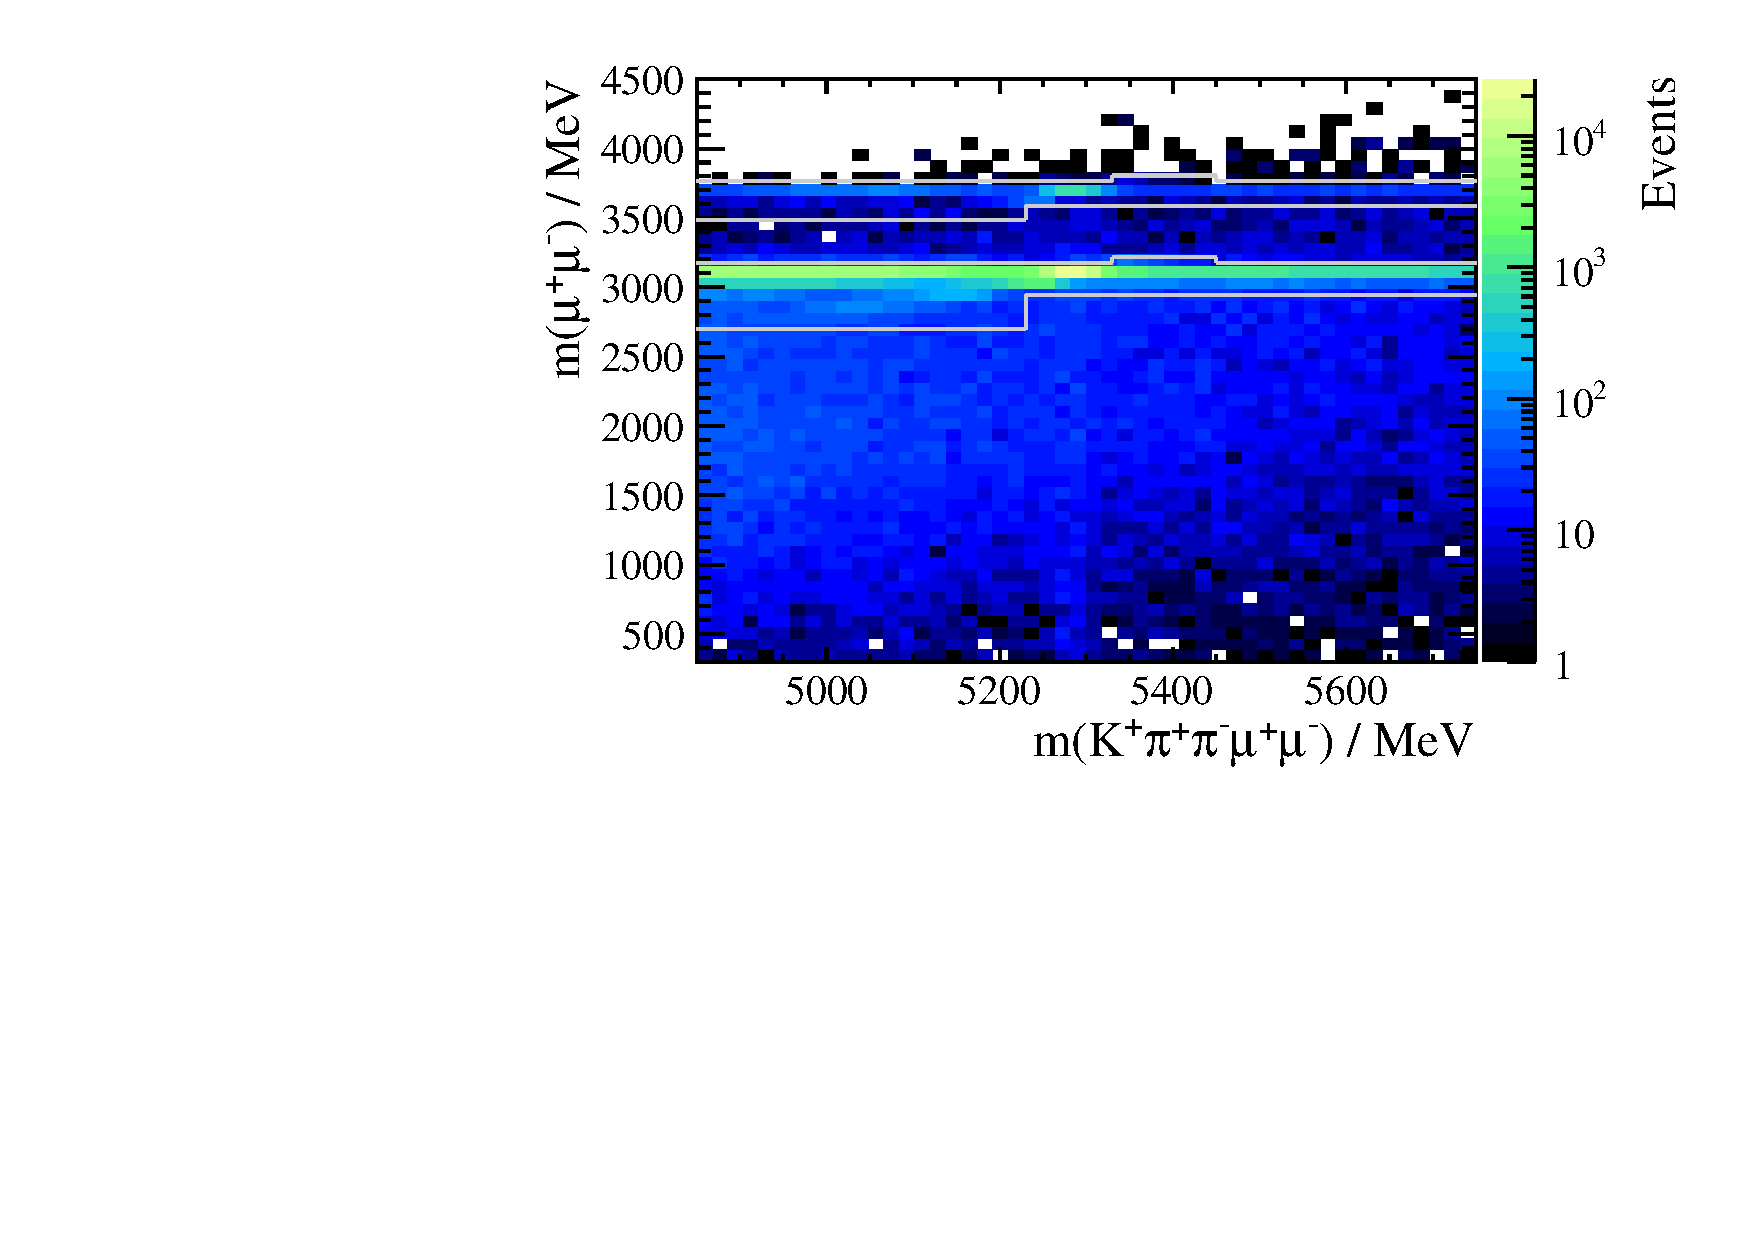
\includegraphics[width=0.48\textwidth]{BvJpost}\\
    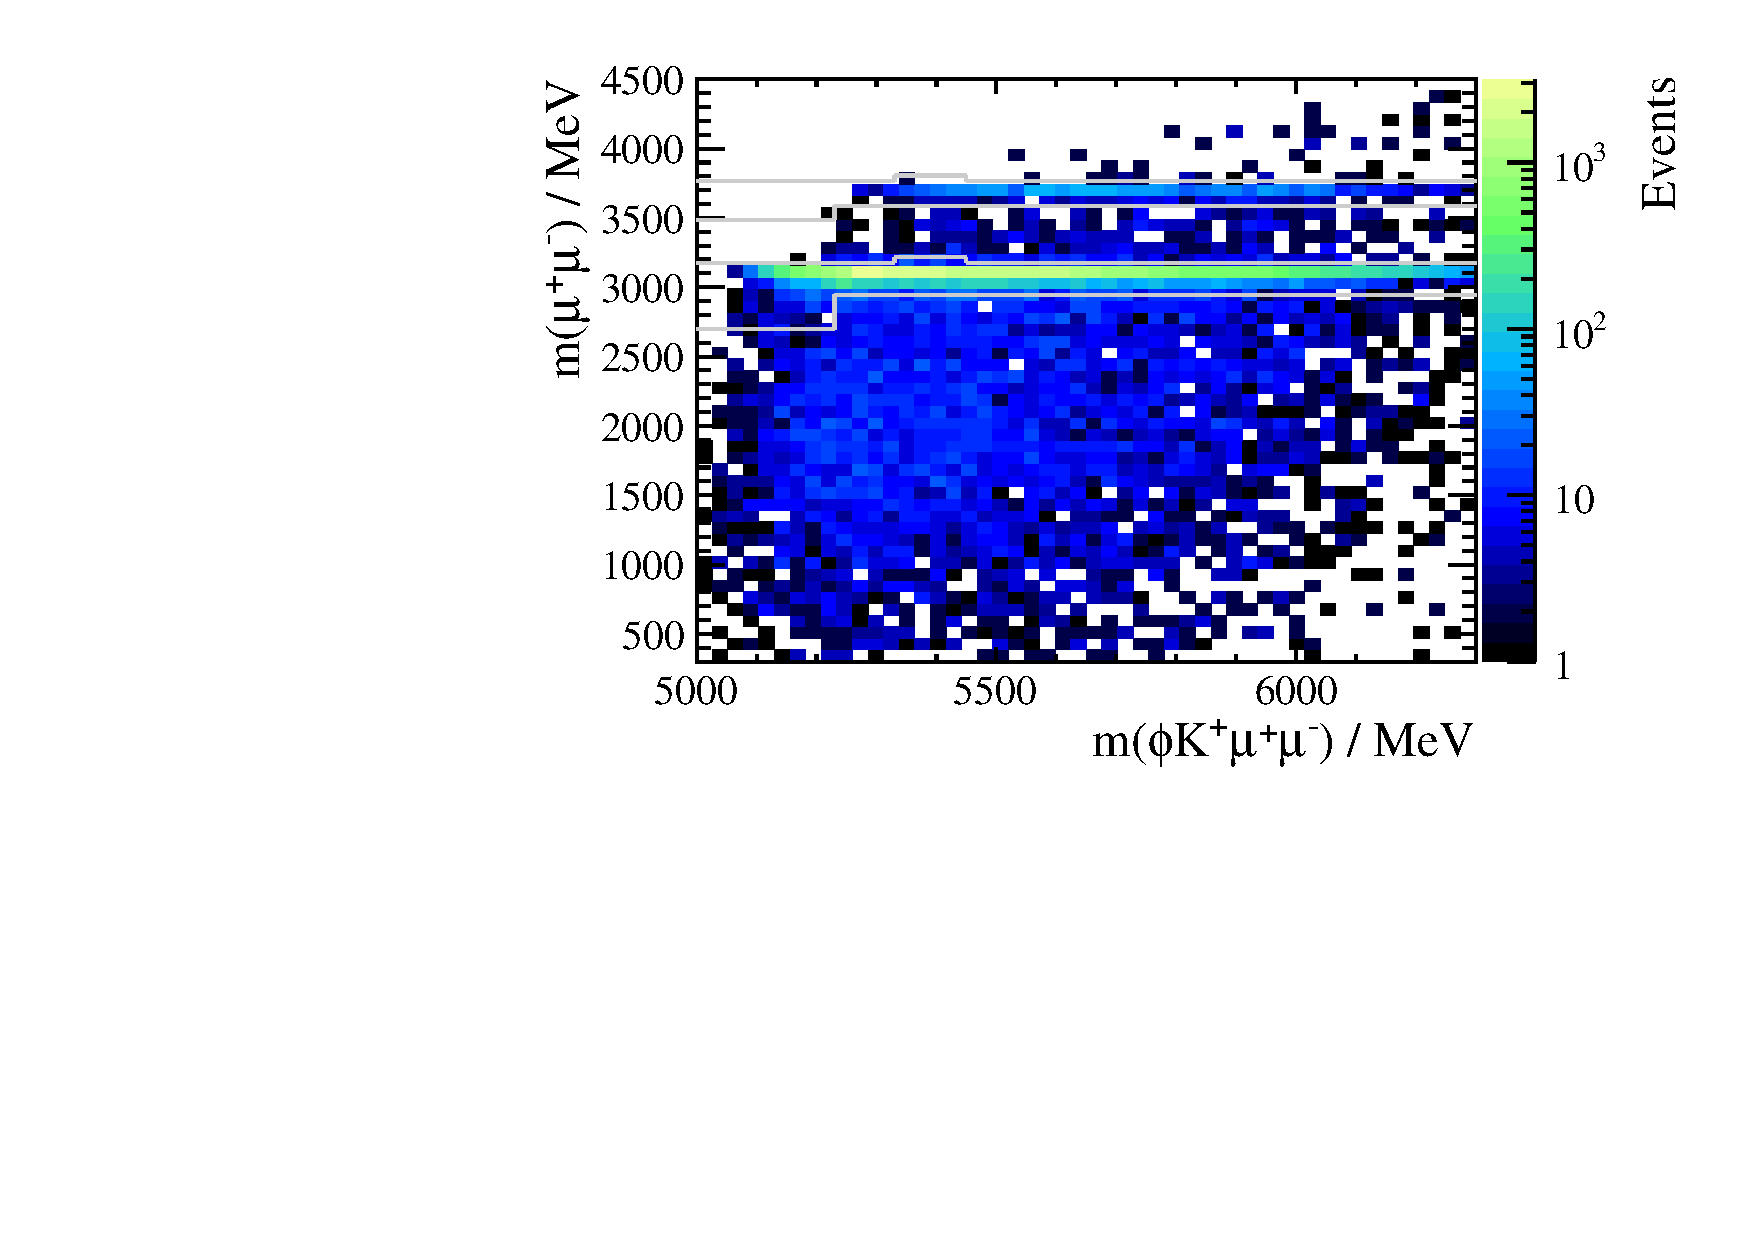
\includegraphics[width=0.48\textwidth]{BvJkkkpre}
    %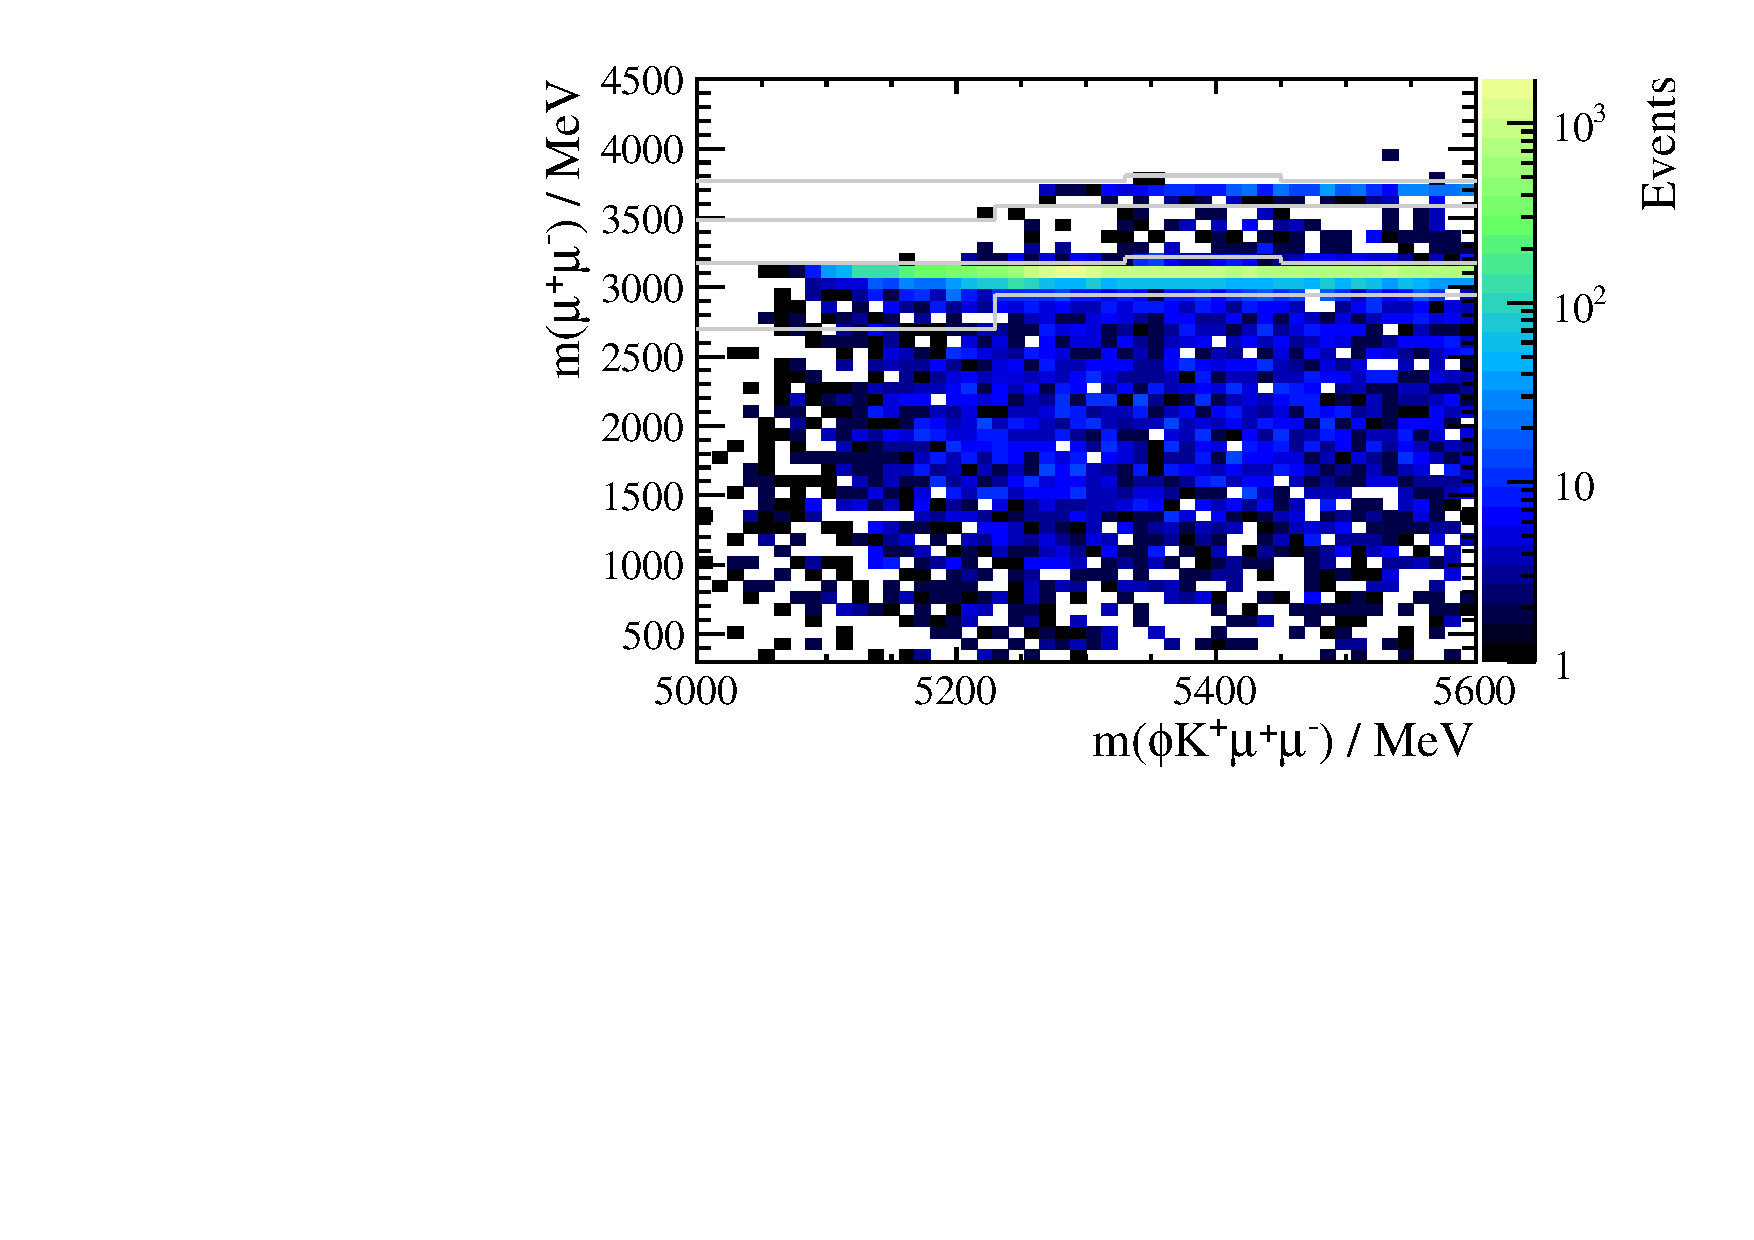
\includegraphics[width=0.48\textwidth]{BvJkkkpost}
    \caption[Charmonium vetoes]
    {\small
      The variation of the invariant mass of the dimuon candidate with the mass of the \Bp
      candidate for
      (left) \btokpipimumu, and
      (right) \btophikmumu.
      The grey lines indicate the boundaries of the charmonium vetoes.
    }
    \label{fig:hhh:charmvetoes}
  \end{center}
\end{figure}

Given the large branching fractions of the charmonium decays given above, and the probability of
misidentifying a muon as a pion is $\mathcal{O}(1\,\%)$,~\cite{LHCb-DP-2013-001}, and slightly less
for kaon, there could have been significant contamination from mis-identified candidates.
This potential background was removed by calculating the invariant mass of each $\mu^+\pi^-$ and
$\mu^+K^-$ combination, where the hadron was assigned the muon mass.
If the mass of this object fell within $50\mev$ of $m_\jpsi$ or $m_\psitwos$, then the candidate
was vetoed.
Figure~\ref{fig:hhh:misid} shows the effect on these vetoes, and demonstrates that a large part
of the background that is removed by these vetoes is from the decay
$\decay{\Bp}{\jpsi\rho(770)^0\Kp}$.


\begin{figure}
  \begin{center}
    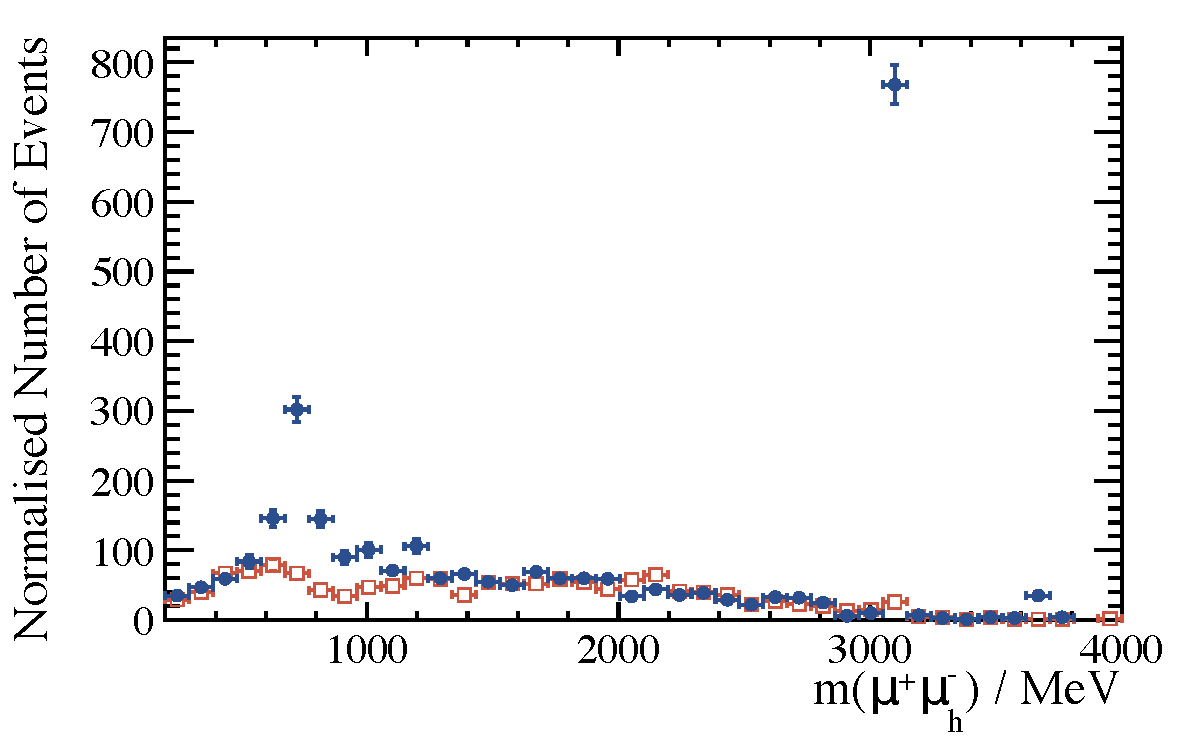
\includegraphics[width=0.45\textwidth]{hhhmisid_pre}
    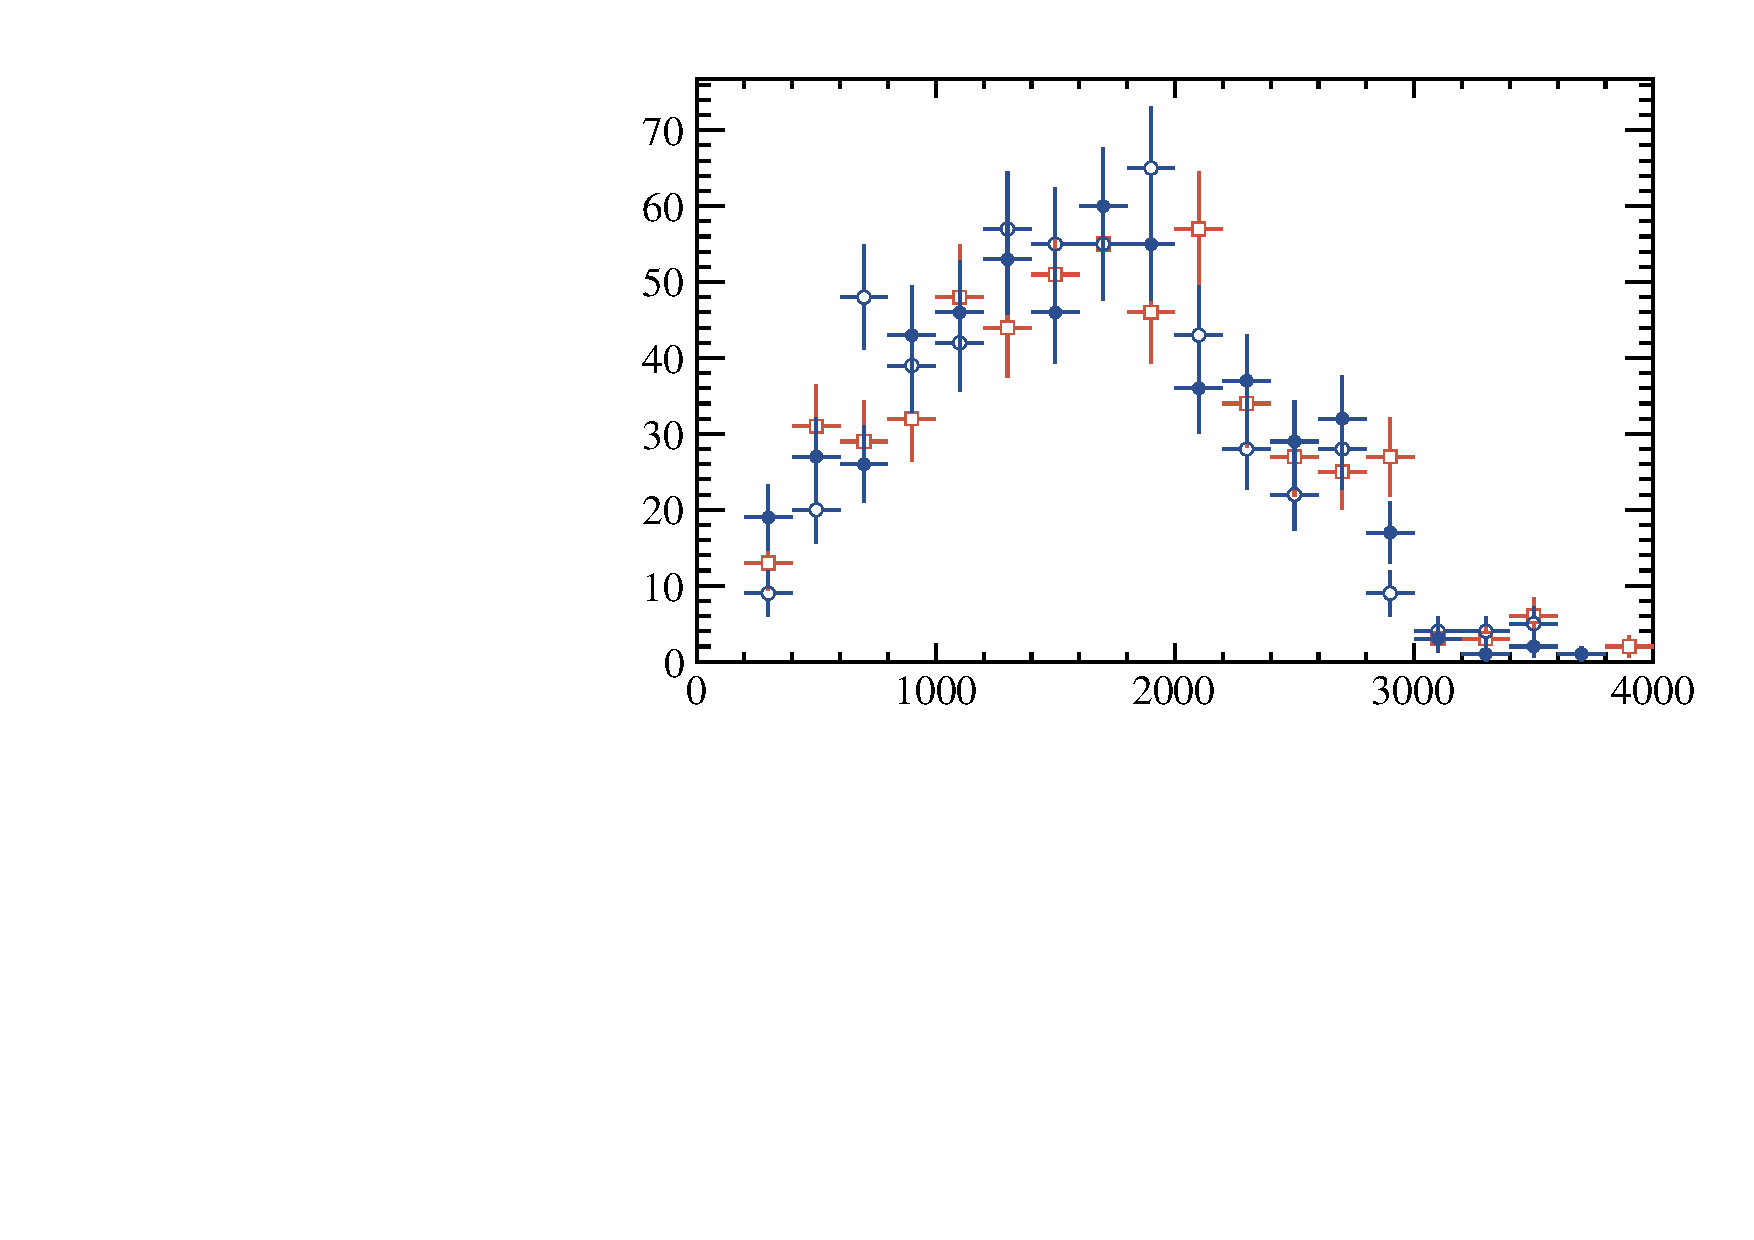
\includegraphics[width=0.45\textwidth]{hhhmisid_post}
    \caption[Backgrounds from misidentified charmonia]
    {\small
      Invariant mass of the combination of a muon and a hadron of the opposite charge
      reconstructed under the muon mass hypothesis.
      The left-hand plot shows the distributions before the veto of misidentification of the \jpsi
      and \psitwos, while the right-hand plot shows the distribution after the vetoes.
      The blue circles are the distribution of $m(\mu\mu\to\mu\pi)$ (solid circles having the same
      charge as the kaon) and red square show the $m(\mu\mu\to\mu K)$ distribution.
      There is a feature at low mass in the $m(\mu\mu\to\mu\pi)$ spectrum which is removed by the
      vetoes, and originates from the background decay $\decay{\Bp}{\jpsi\rho(770)^0\Kp}$.
    }
    \label{fig:hhh:misid}
  \end{center}
\end{figure}

\begin{figure}[h]
  \begin{center}
    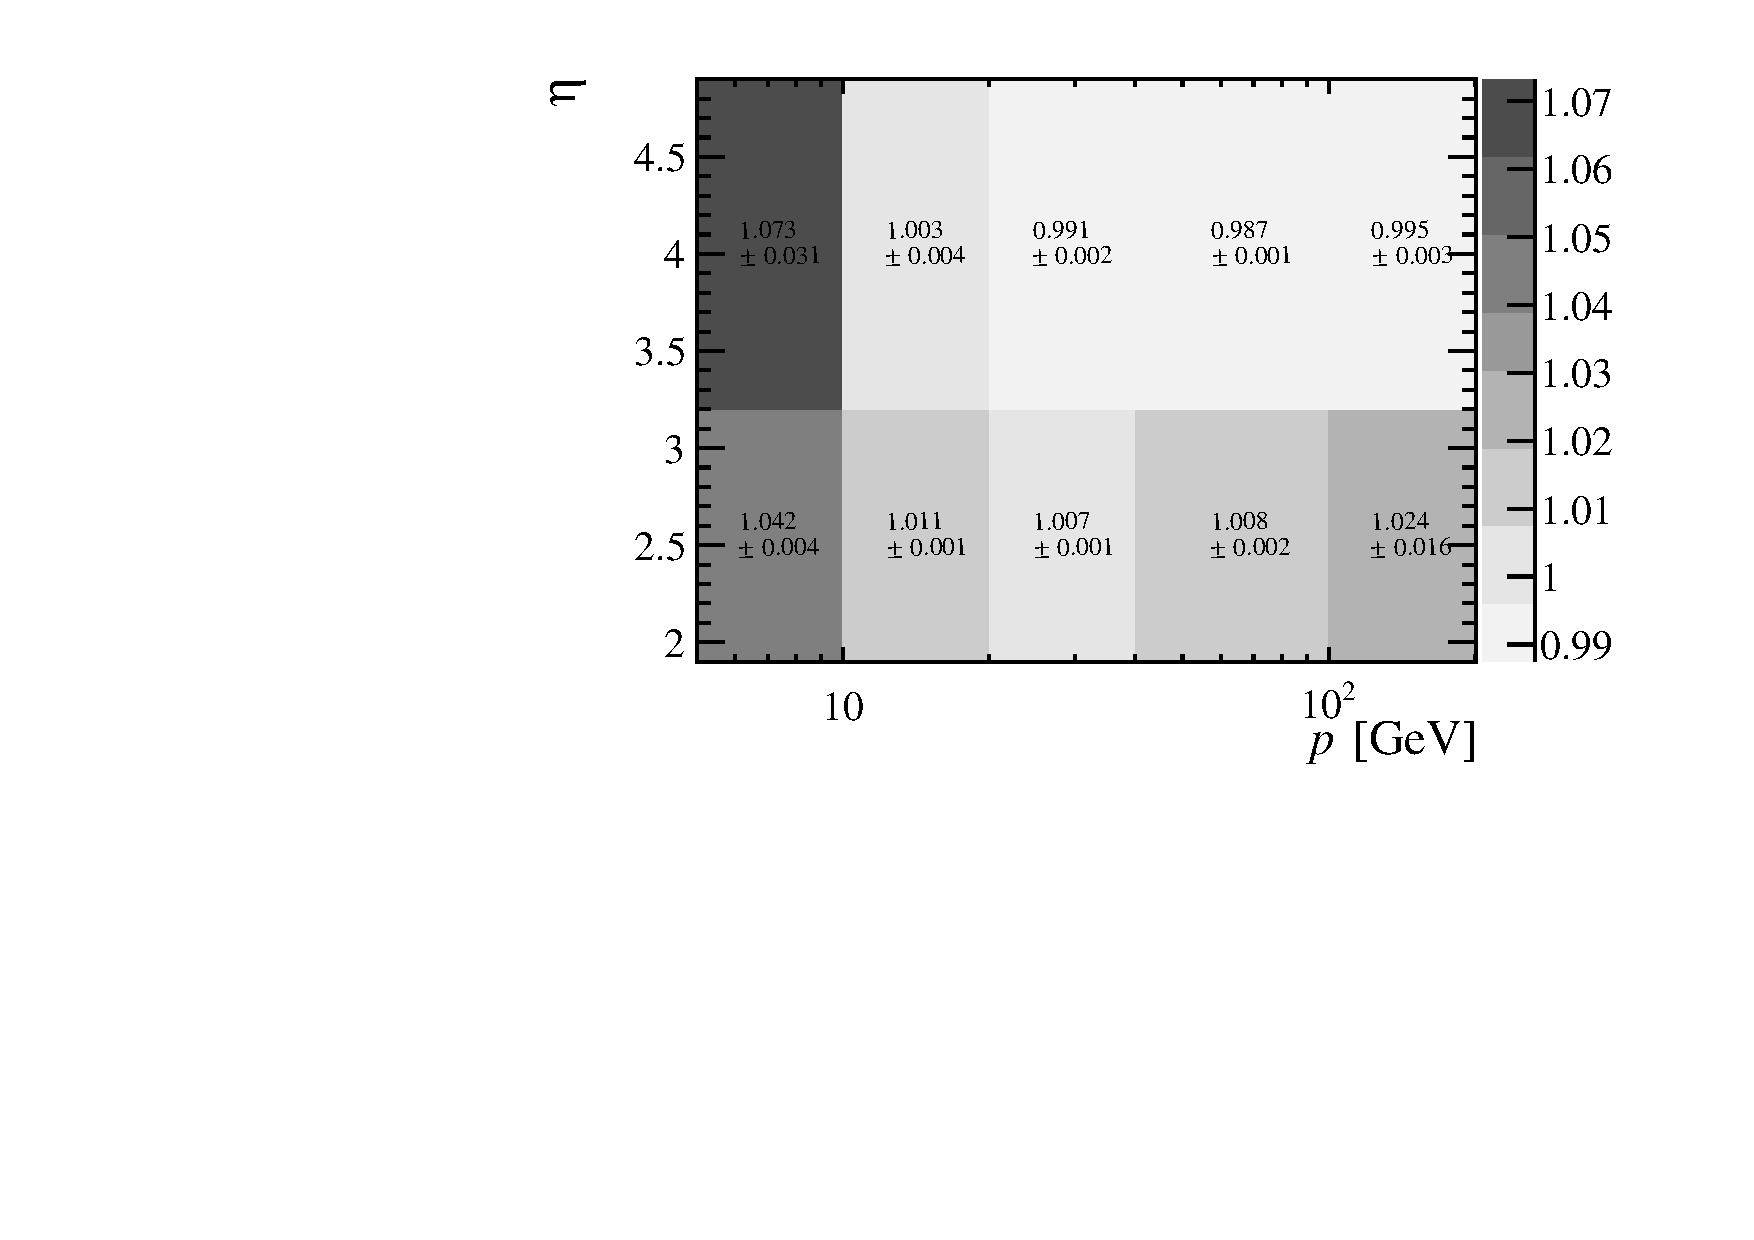
\includegraphics[height=0.23\textheight]{trackeff}
    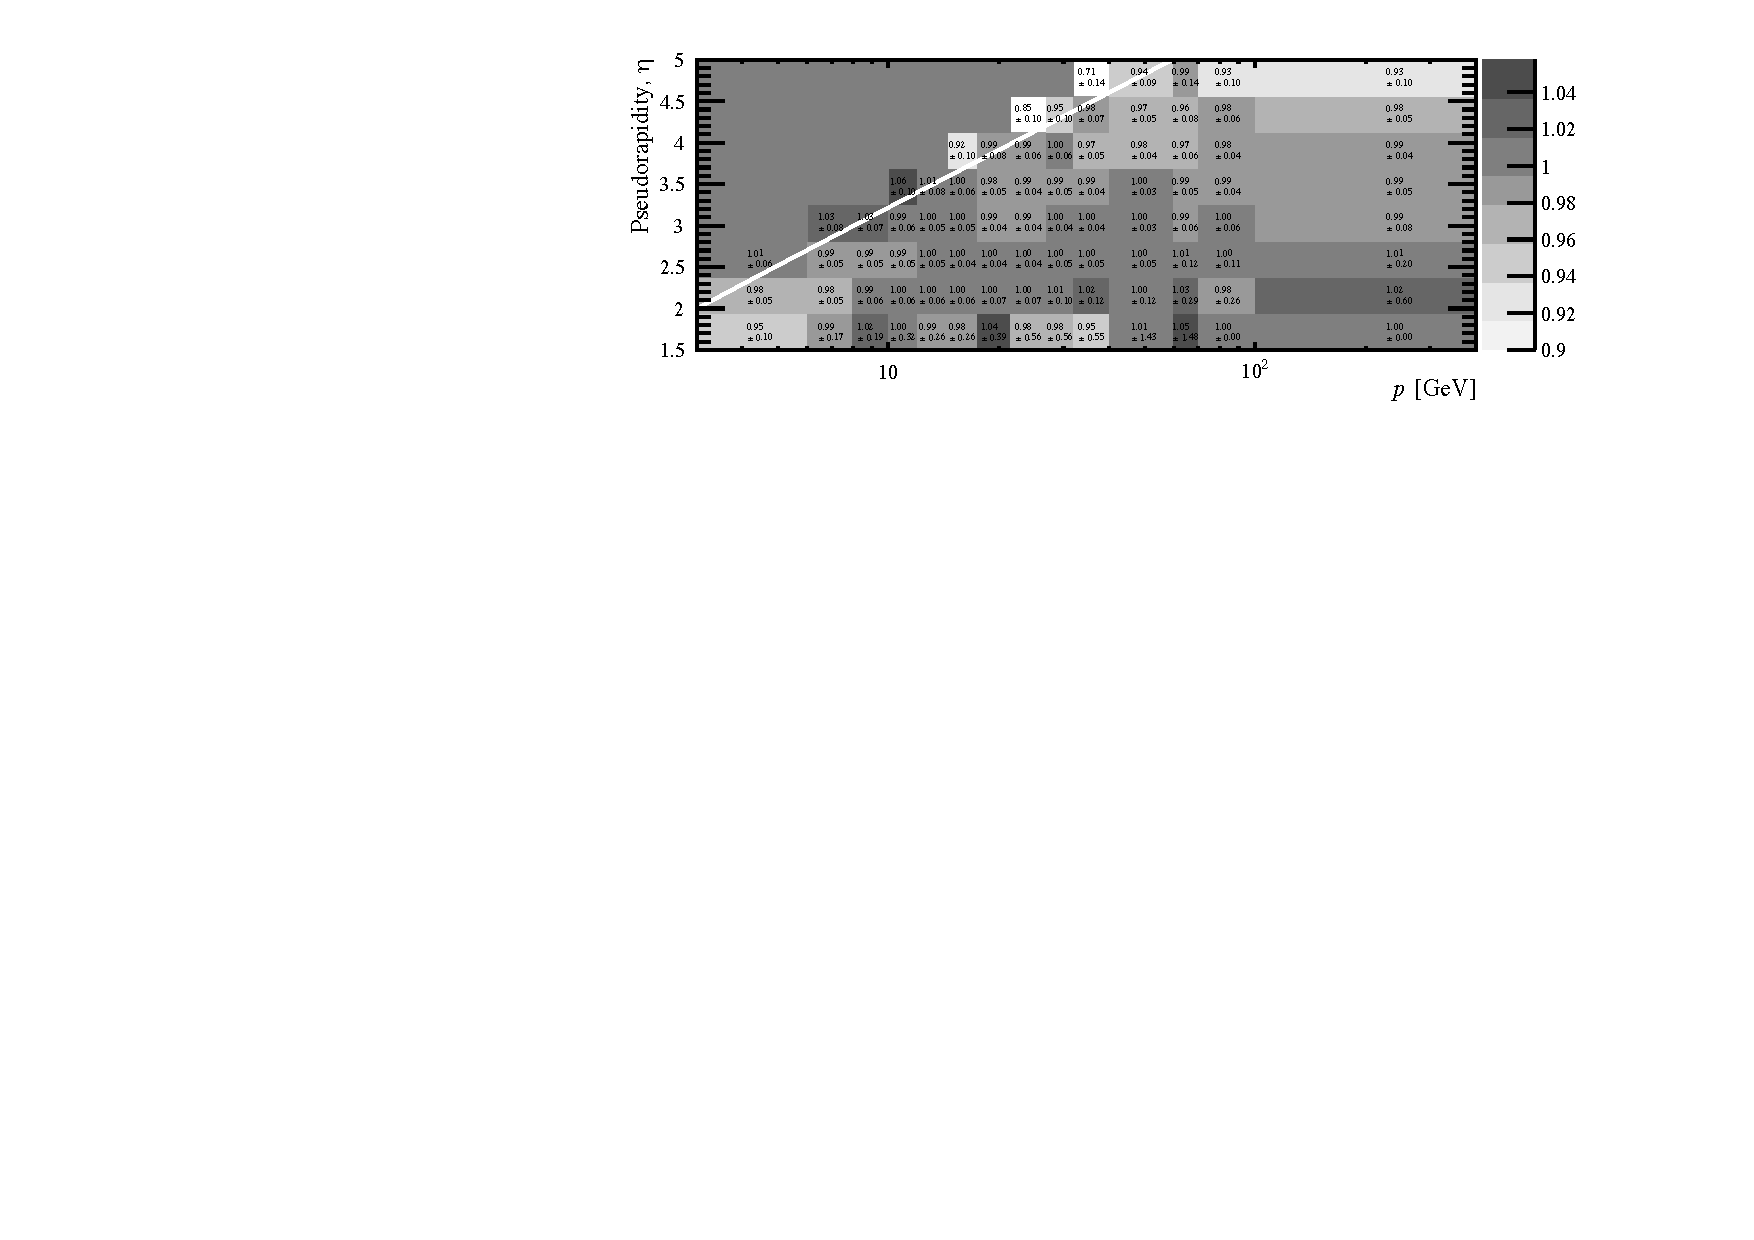
\includegraphics[height=0.23\textheight]{muoneff}
  \end{center}
  \caption{
    The ratio of efficiencies for (top) tracking, and (bottom) \ismuon between data and simulation.
    Simulated tracks in simulation are reweighted according to their momentum and $\eta$.
    For the lower plot, the calibration sample does not contain muons with $\pt<800\mev$, this
    geometric threshold is indicated by the white line.
  }
  \label{fig:hhh:trackeff}
\end{figure}

Other peaking backgrounds D0...


Semileptonic cascades, where a \bquark decays via $\decay{b}{c\mun\bar\nu_\mu}$ and subsequently
$\decay{c}{s\mup\nu_\mu}$, can have branching fractions as high as $\mathcal{O}(10^{-4})$.
For example, the decay $\decay{\Bp}{\Dm\pip\mup\nu_\mu}$ followed by
$\decay{\Dm}{\Kp\pim\mun\bar\nu_\mu}$ has a total branching fraction of
$(1.6\pm0.3)\e{-4}$~\cite{PDG2014}.
Selection requirements on the \chisqvtx suppress these decays significantly, and the energy lost to
the neutrinos means that this background peaks considerably below the known \Bp mass.




\subsection{Multivariate selection}
\label{sec:hhh:bdt}
Combinatorial background was suppressed using a BDT trained using the AdaBoost
algorithm~\cite{AdaBoost}, which is described in detail in \Chap{sec:bdt:ada}.
Both signal and background samples used for BDT training were taken from data.
The sample of data used as the signal-proxy was from  the decay \btojpsikpipi, which had been
\emph{sWeighted}~\cite{splot} for the purpose of removing combinatorial background from the
training sample.
For the background sample, selected signal mode data was taken from the upper mass sideband of the
\Bp candidate mass, in the range $5530<m_{K\pi\pi\mu\mu}<5780\mev$.
These candidates are not used for the determination of the signal yield, and at this high mass are
comprised solely of combinatorial background.

This BDT was trained using selection of geometric and kinematic variables, the exact variables are
listed in \Tab{hhh:tab:bdtvars}.

\begin{table}
  \caption[BDT training variables]
  {\small
    Input variables used to train the BDT to distinguish between signal \btokpipimumu decays and
    combinatorial backgrounds.
  }
  \label{hhh:tab:bdtvars}
  \begin{center}
    \begin{tabular}{lc}\\\toprule
      Particle & Variable\\\midrule
      \Bp & \pt\\
      & \chisqip \\
      & \chisqfd\\
      & \chisqvtx\\
      & $\theta_\mathrm{dir}$\\\littlerule
      Tracks & \pt\\
      & \chisqip\\
      %\hline
      \bottomrule
    \end{tabular}
  \end{center}
\end{table}


\subsubsection[Optimization of \btokpipimumu cuts]
{Optimization of \tmath{\btokpipimumu} cuts}
\label{sssec:opt:kpipi}
The determination of the optimum cut value on the BDT was made in conjunction with optimizing PID
criteria on each hadron.
For the decay \btokpipimumu, a requirement that $\dllkpi(\Kp)-\dllkpi(\pip)>10$ was made, this
simply ensured that of the two hadrons with the same sign, the one identified as a kaon had more of
a kaon like signature than the other.
Then, optimization was made in the three dimensions of BDT, $\dllkpi(\Kp)$ and $\dllkpi(\pi^\pm)$
by maximising the figure of merit $S/\sqrt{S+B}$, where $S$ and $B$ are the expected signal and
background yields respectively.
The value of $S$ was determined by scaling the weighted sum of selected \btojpsikpipi events,
$N\big(\jpsi\kpipi\big)$, according to
\begin{equation}
  S =
  \frac{
    \BF\big(\decay{\Bp}{\kone{1270}\mumu}\big)
    \BF\big(\decay{\kone{1270}}{\kpipi}\big)
  }{
    \BF\big(\decay{\Bp}{\jpsi\kpipi}\big)
    \BF\big(\decay{\jpsi}{\mumu}\big)
  }
  \cdot
  N\big(\btojpsikpipi\big).
\end{equation}
Where, branching fraction values used in this calculation are taken to be
$\BF\big(\decay{\kone{1270}}{\kpipi}\big) = 35.7\,\%$~\cite{PDG2012},
$\BF\big(\jpsitomumu\big) = 5.93\,\%$~\cite{PDG2012} and
$\BF\big(\btojpsikpipi\big) = 8.1\e{-4}$~\cite{PDG2012}.
Estimation of the branching fraction of the signal decay \decay{\Bp}{\kone{1270}\mumu} is made
assuming the ratio of the branching fractions for the known decays \decay{B}{X\mumu} to
\decay{B}{X\mumu}
is the same for $X$ being the \kone{1270} or \Kstarent.
Thus,
\begin{align}
  \BF\big(\decay{\Bp}{\kone{1270}\mumu}\big)
  &=
  \BF\big(\decay{\Bp}{\kone{1270}\gamma}\big)
  \cdot\frac{
    \BF\big(\decay{\Bp}{K^*(892)^0\mumu}\big)
  }{
  \BF\big(\decay{\Bp}{K^*(892)^0\gamma}\big)
  }\nonumber\\
  &=\big(1.05\pm0.34\big)\e{-6}.
\end{align}

%This optimization was performed using the cross-check channel \btojpsikpipi, where $S$ was defined
%as the weighted sum of events that pass a given set of cuts, and $B$ was
%where $S$ is defined as the

The value of the estimated background yield, $B$, was determined from interpolating signal
\btokpipimumu candidates from the sidebands into the mass regions around the mass of the \Bp meson.
Candidates falling in the low and high mass sidebands
(defined by $5000<m_{K\pi\pi\mu\mu}<m_{\Bp}^\pdg-120\mev$ and
$m_{\Bp}^\pdg+120<m_{K\pi\pi\mu\mu}<5750\mev$ respectively),
were fitted to an exponential, and the value of $B$ was taken to be the integral of this
distribution within $60\mev$ of the known \Bp mass~\cite{PDG2012}.

The maximum value of the figure of merit
was found (as shown in \Tab{tab:hhh:opt}), and corresponding cut values used for the analysis.
The exact requirements for the PID were that $\dllkpi(\Kp)>3.5$, $\dllkpi(\pi^\pm)<14.5$ and
$\mathrm{BDT}>0.025$.

\begin{figure}
  \begin{center}
    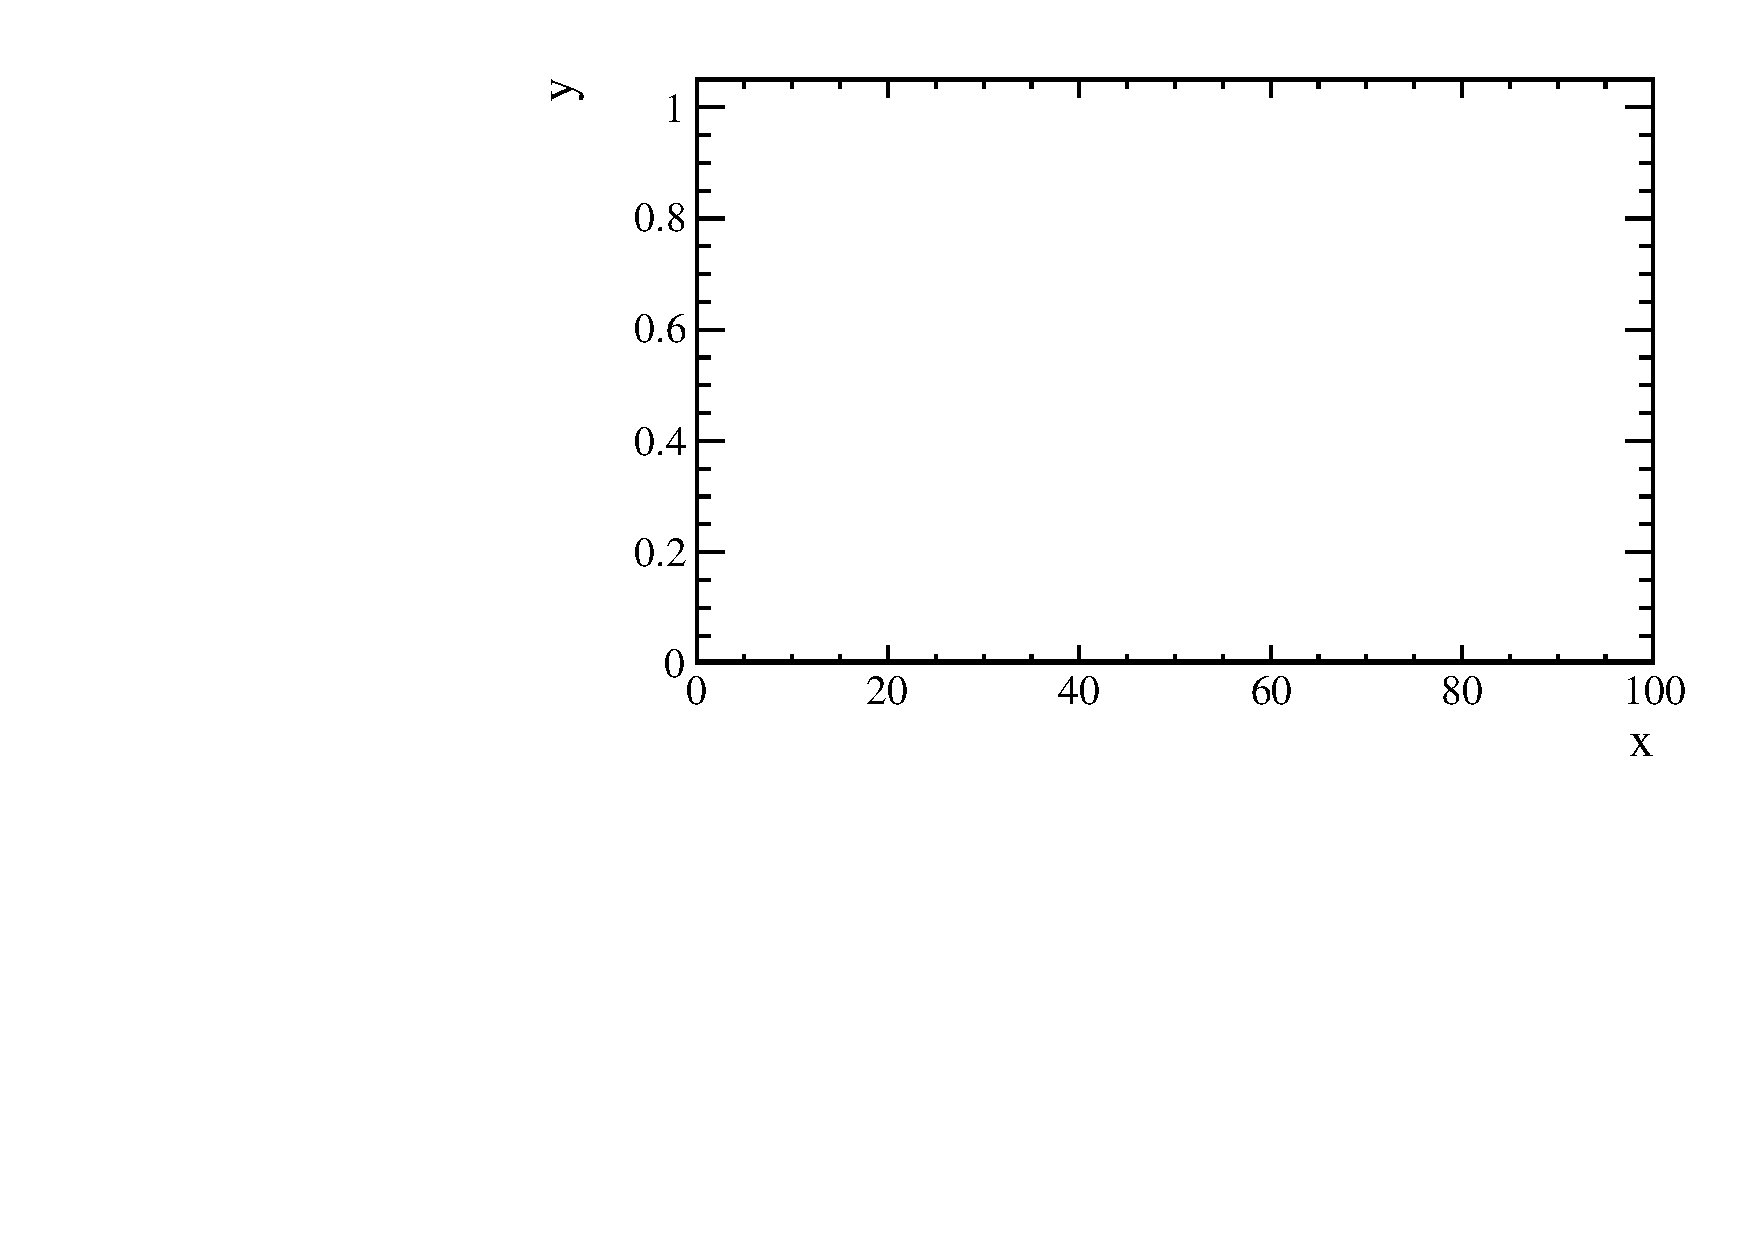
\includegraphics[width=0.48\textwidth]{blank}
    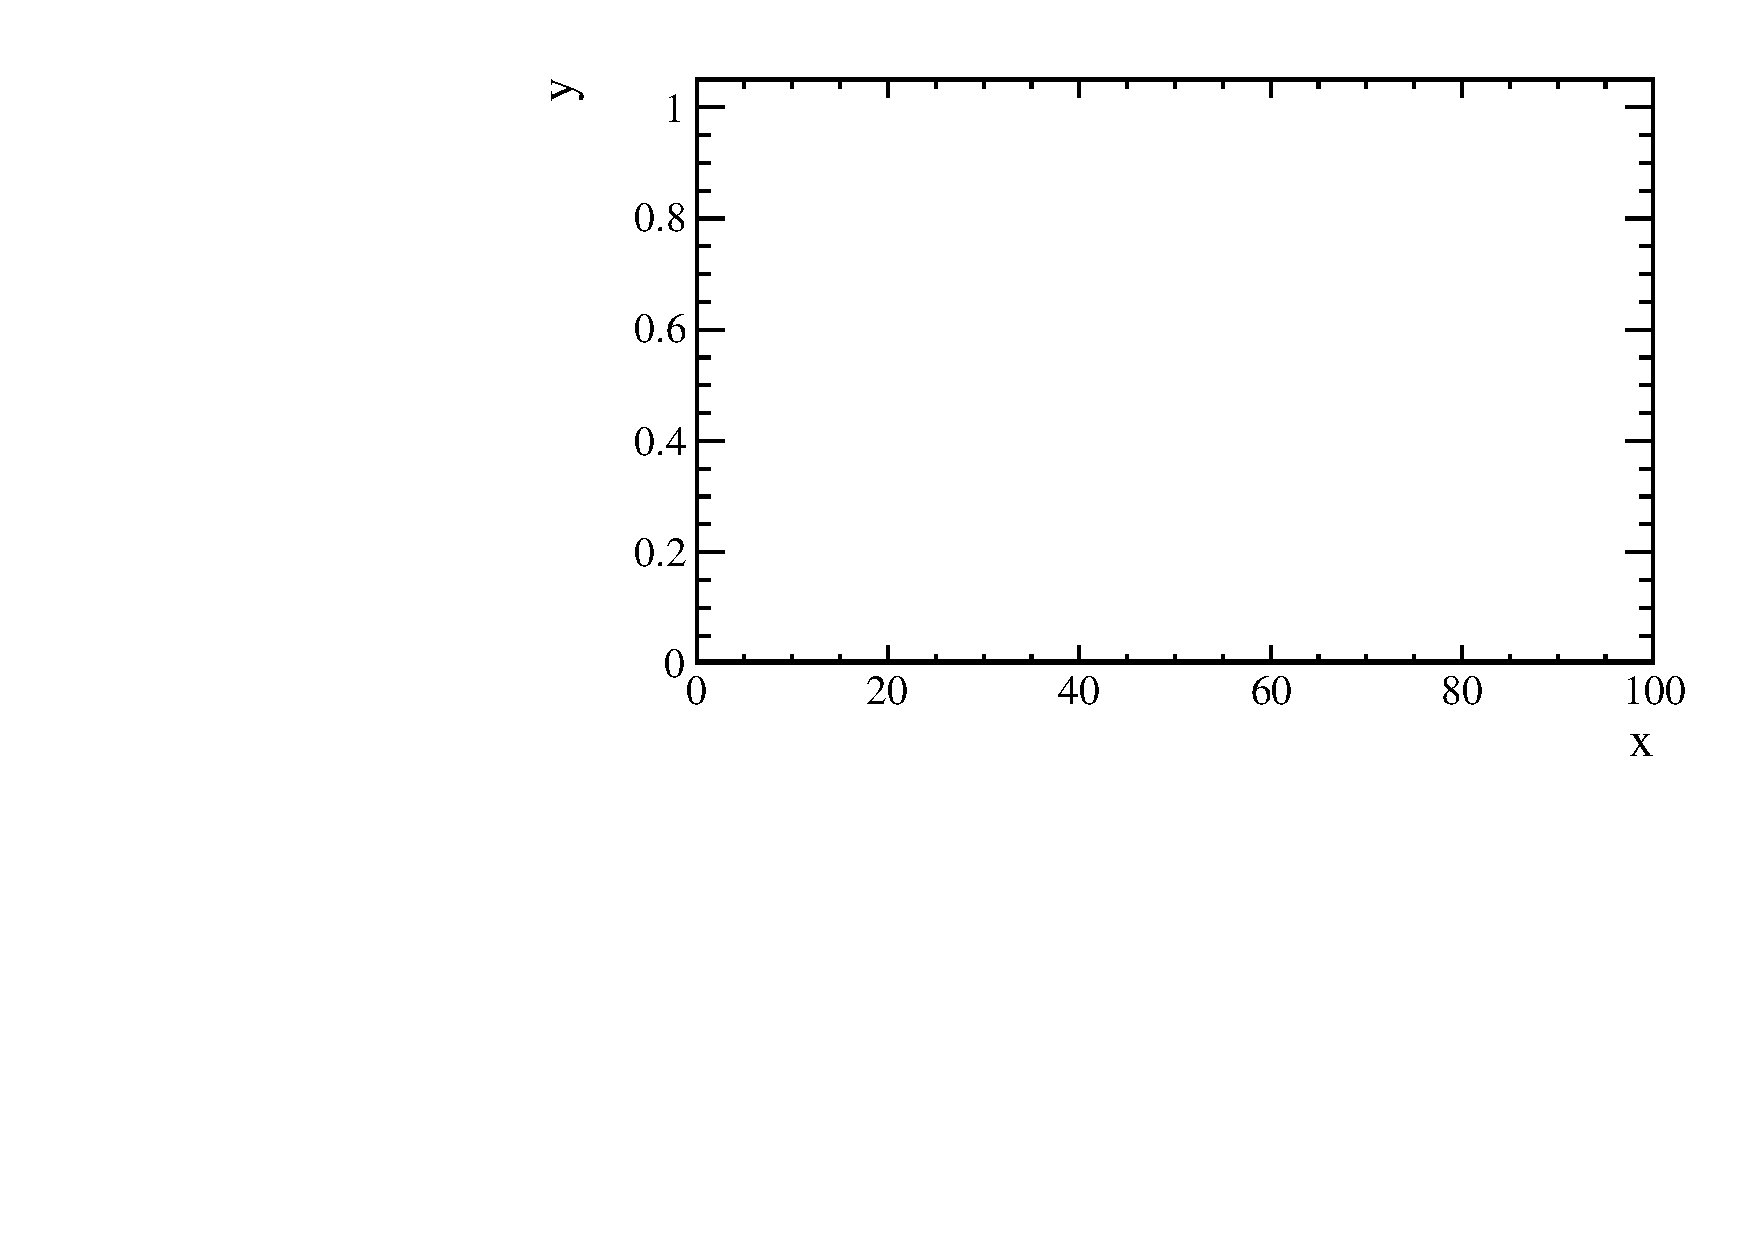
\includegraphics[width=0.48\textwidth]{blank}
    \caption{\small
      FILL IN.
    }
    \label{fig:kpipi:opt}
  \end{center}
\end{figure}


\subsubsection[Optimization of \btophikmumu cuts]
{Optimization of \tmath{\btophikmumu} cuts}
This channel follows a similar procedure for optimization as for the decay \btokpipimumu.
Optimization was performed in multiple dimensions (BDT and $\dllkpi(K^\pm)$) with the chosen
selection of cuts maximizing the figure of merit $S/\sqrt{S+B}$.
The calculation of $B$ was made in the same way as described above, and the
value of $S$ was determined in a similar way, by scaling the \emph{sWeighted} sum of candidates
that passed given cuts by the ratio of known branching fractions.
Therefore,
\begin{equation}
  S =
  \frac{
    \BF\big(\decay{\Bp}{\phi\Kp\mumu}\big)
  }{
    \BF\big(\decay{\Bp}{\jpsi\phik}\big)
    \BF\big(\decay{\jpsi}{\mumu}\big)
  }
  \cdot
  N\big(\jpsi\phi\Kp\big).
\end{equation}
where $N\big(\jpsi\phik\big)$ is the weighted number of selected \btojpsiphik events.
The expected background yield is determined using an exponential fit across the signal region, as
is done for the \btokpipimumu channel.
The prediction for the branching fraction of the signal channel is taken to be
\begin{align}
  \BF\big(\decay{\Bp}{\phi\Kp\mumu}\big)
  &=
  \BF\big(\decay{\Bp}{\phi\Kp\gamma}\big)
  \cdot\frac{
    \BF\big(\decay{\Bp}{K^*(892)^0\mumu}\big)
  }{
    \BF\big(\decay{\Bp}{K^*(892)^0\gamma^{}}\big)
  }\nonumber\\
  &=\big(0.66\pm0.12\big)\e{-7}.
\end{align}
Figure~\ref{fig:phik:opt} shows the variation of the figure of metric for different values of the
BDT and $\dllkpi(K)$ cuts, the optimal values are given in \Table{tab:hhh:opt}.

\begin{figure}
  \begin{center}
    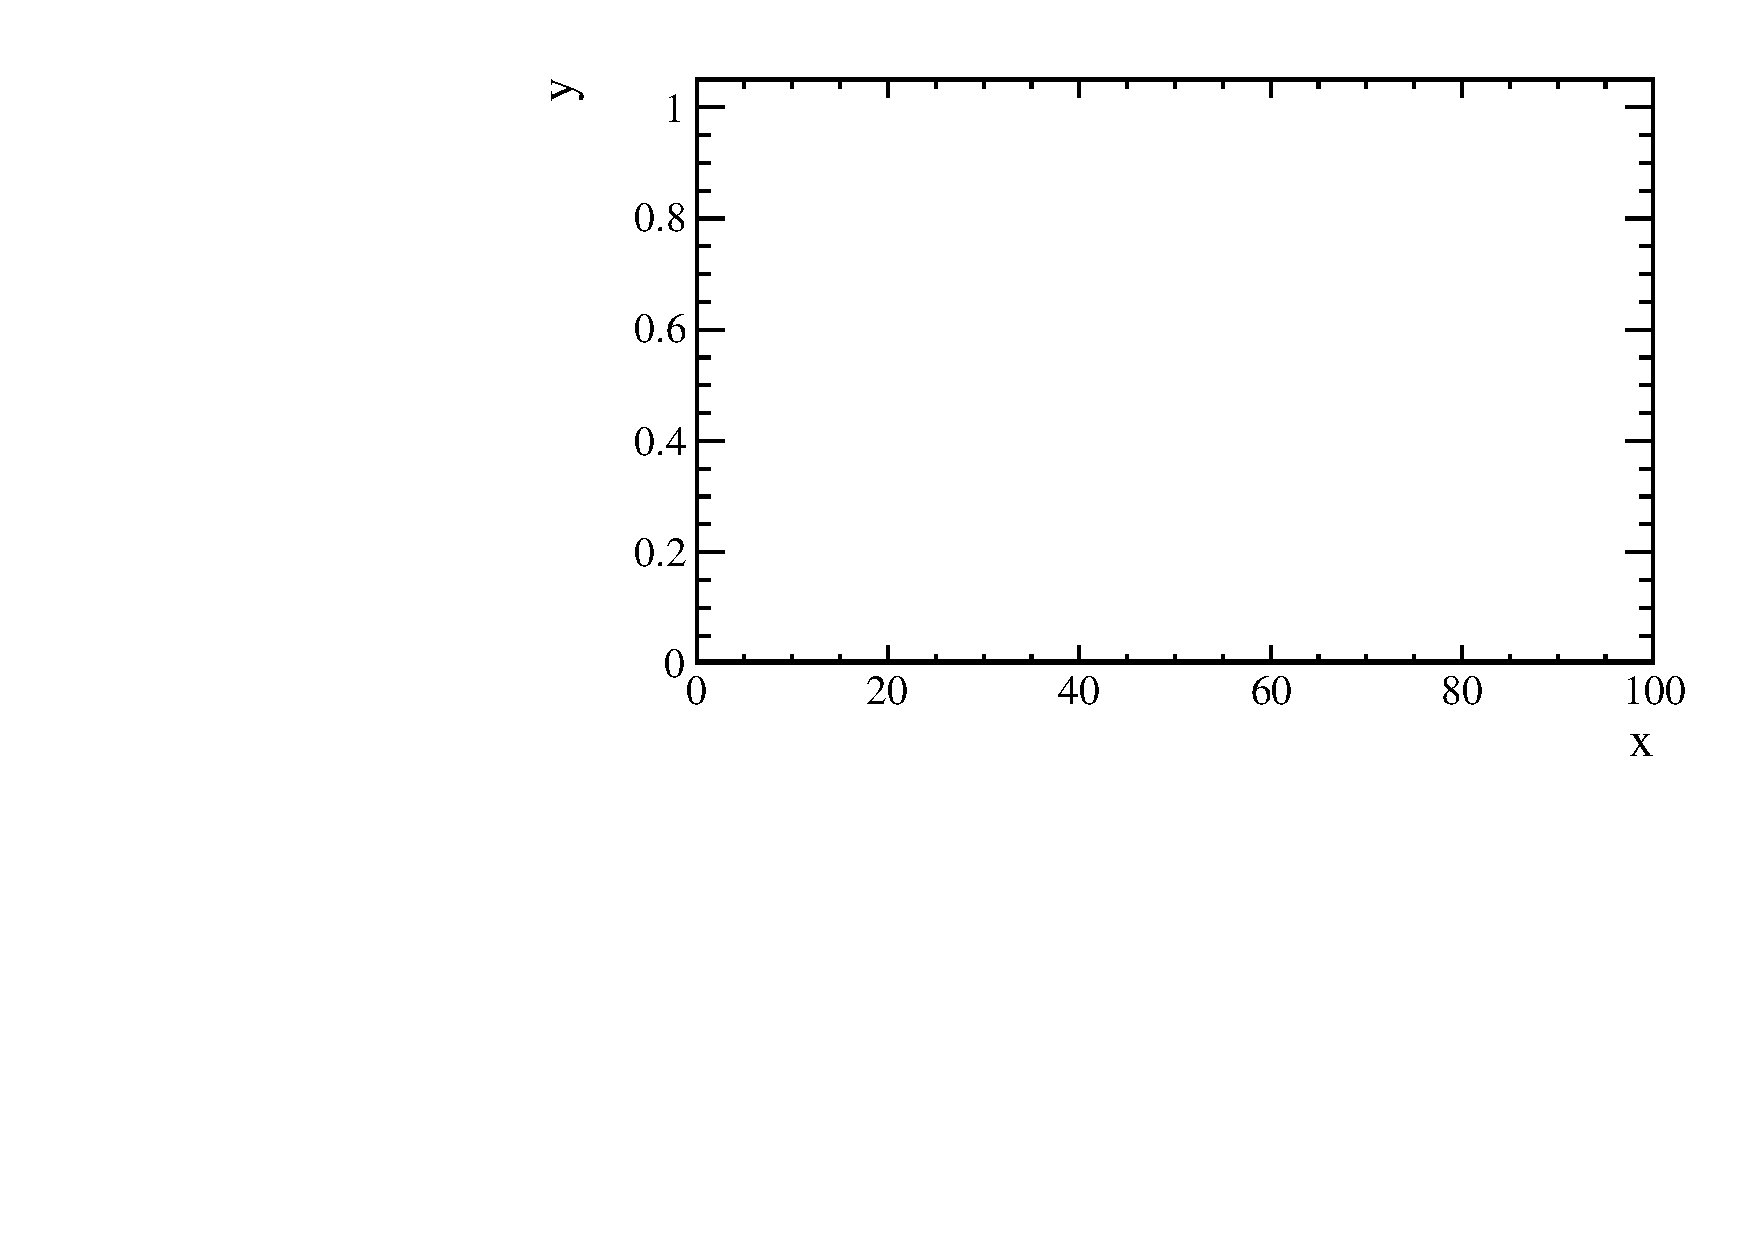
\includegraphics[width=0.48\textwidth]{blank}
    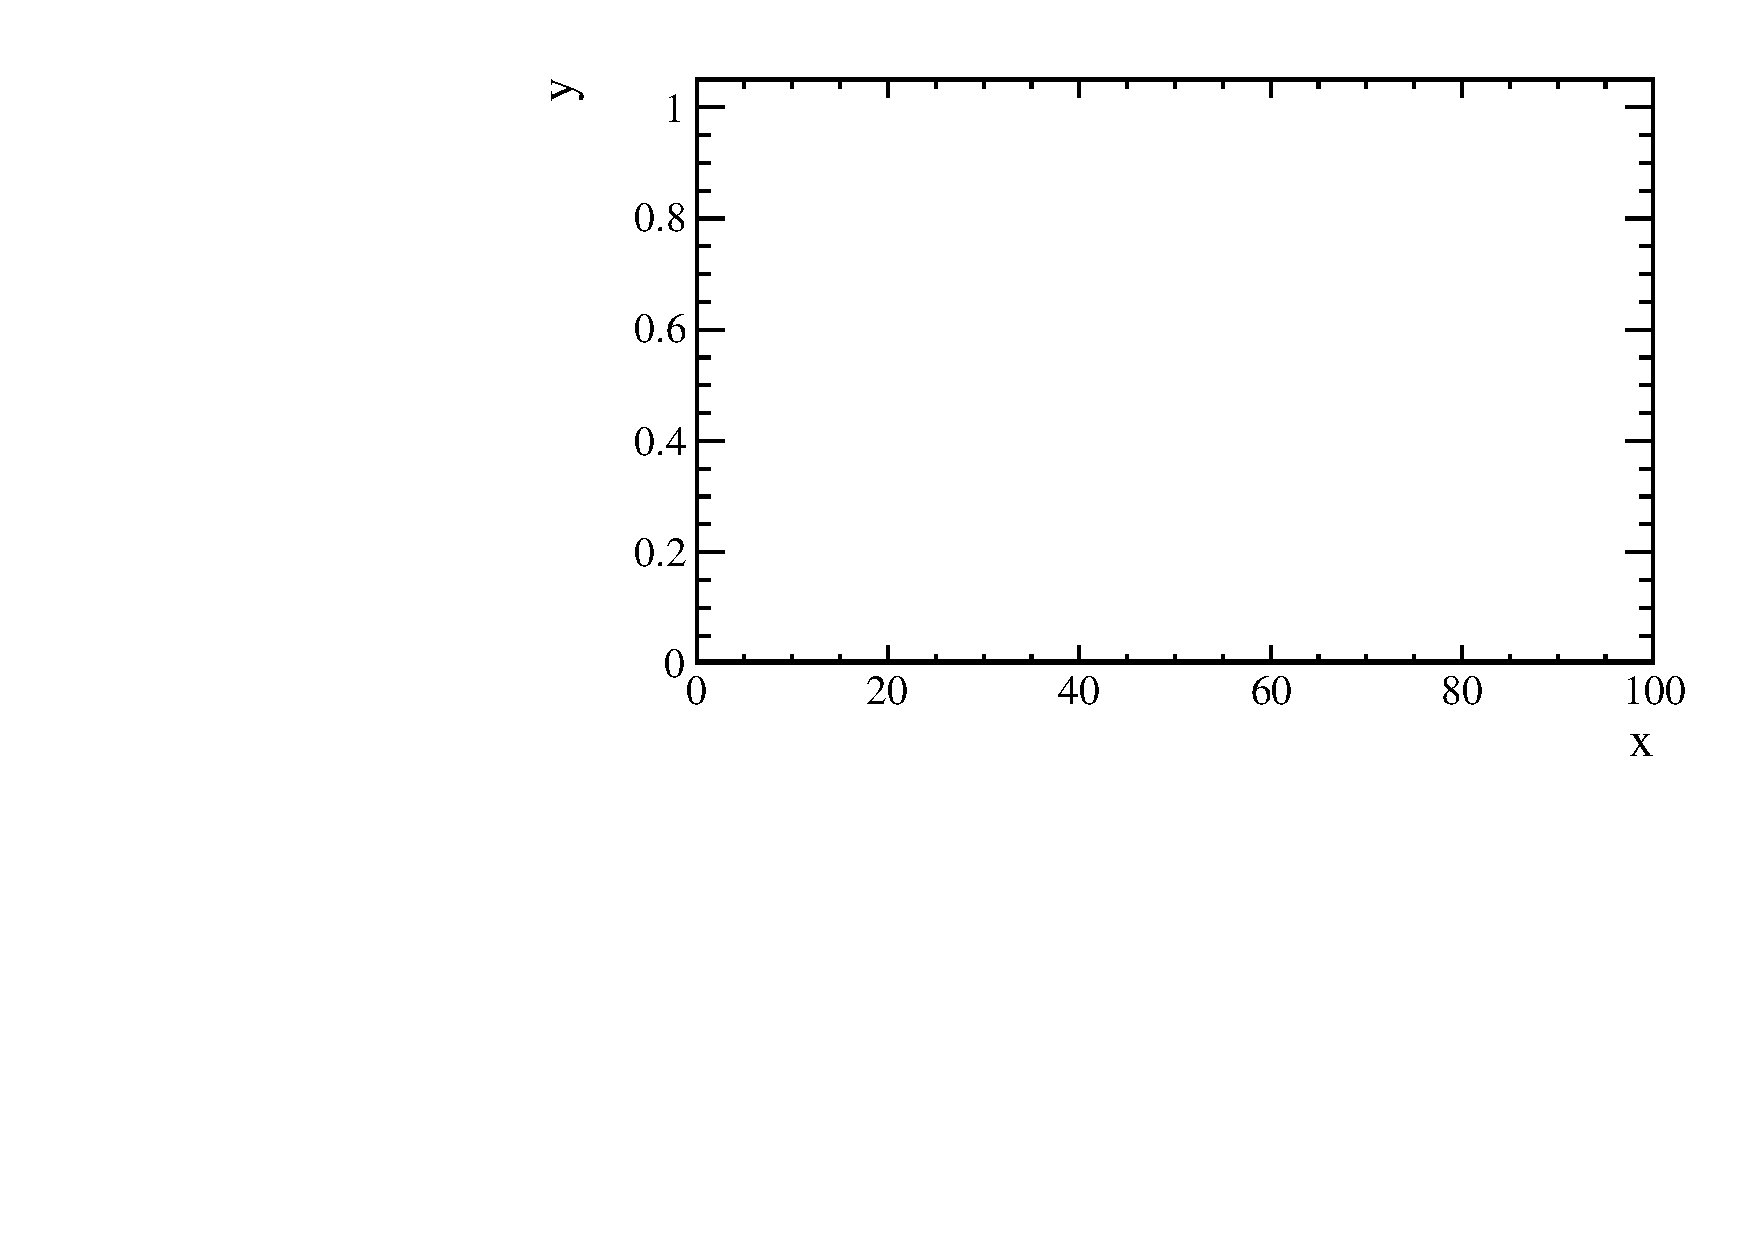
\includegraphics[width=0.48\textwidth]{blank}
    \caption{\small
      FILL IN.
    }
    \label{fig:phik:opt}
  \end{center}
\end{figure}

%\begin{table}
  %\caption[Expected yields]
  %{\small
    %Expected values for $S$ and $B$ for the maximum value of the figure of merit $S/\sqrt{S+B}$.
    %These are taken from the 2012 sample only.
  %}
  %\label{tab:hhh:opt}
  %\begin{center}
    %\begin{tabular}{lrrc}\toprule
      %\cellc{Decay} & \cellc{$S$} & \cellc{$B$} & \cellc{$S/\sqrt{S+B}$} \\
      %\midrule
      %\btokpipimumu & 304 & 166 & 14.0 \\
      %\btophikmumu  &  28 &   8 & \pz4.7 \\
      %\bottomrule
    %\end{tabular}
  %\end{center}
%\end{table}







%\subsection{Reweighting of variables}


%\section{Backgrounds}
%\section{Mass fits}
%\section{Efficiencies}
%\section{Systematics}
%\section{Summary}

%PID info from the RICH is used to identify final state hadrons
%PV chosen based on lowest PV of B candidateo
%vertex fit \chisq must increase by more than 121 when including the B candidate daughters
%fit vertex chi2 < 6
%Backgorunds of \jpsi and \psitwos must be removed
%also their radiative tails
%main sources of peaking backgrounds come from charmonia
